\documentclass[a4paper, 12pt,oneside]{article} 
%\documentclass[a4paper, 12pt,oneside,draft]{article} 

\usepackage{preamble}
\usepackage{bm}

%--------------------- ACTUAL FILE ---------------------- %
\begin{document} 
	\begin{center}
	    \Large
	    \textbf{RL mini-project : Mountain Car environment}
	        
	    \vspace{0.4cm}
	    \large
	    Authors : Rayan Harfouche \& Tara \footnote[1]{My administrative name is Tobia, so you will find me under that name in EPFL related databases.} Fjellman \\
	    \small{Spring 2024}
	\end{center}

    \section{Introduction}
        To be written after the rest of the report is done.

    \section{Environment}
        The Mountain Car environment is a classic reinforcement learning problem. The agent is placed in a valley between two hills and has to learn to reach the top of the right hill. The agent can only apply a force of -1, 0 or 1 to the car. The car has a maximum speed of 0.07 and a maximum position of 0.6. The agent receives a reward of -1 at each time step, and a reward of 0 when it reaches the top of the hill. The episode ends when the agent reaches the top of the hill or after 200 steps. The state space is continuous and has two dimensions, the position and the velocity of the car. The action space is discrete and has three dimensions, the force applied to the car. The environment is implemented in the OpenAI gym library.
    \section{Random agent}
    \begin{wrapfigure}{r}{0.6\textwidth}
        \centering
        \vspace{-1em}
        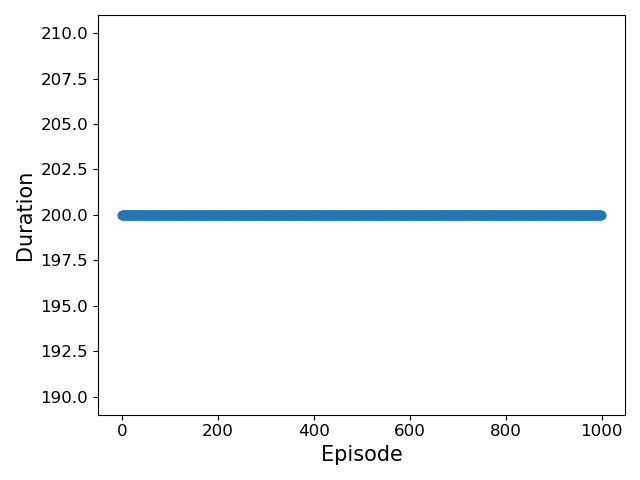
\includegraphics[width=0.6\textwidth]{../runs/random/n_eps=1000/figs/duration}
        \caption{Episode duration of random agent during training.}
        \label{fig:random-neps=1000}
    \end{wrapfigure}
    To analyse the performance of the agent, one can analyse the duration of the episodes as a function of time. Indeed, if the agent learns the task, the duration of the episodes should decrease in time. This because at the start the agent doesn't know the task, and so the episode is truncated at `full\_ep\_len=200', while as it learns it, it should manage to finish the task before reaching the step limit.
    Running the the agent for 100 episodes, we obtain fig ... . Looking at it, it is clear that the agent does not learn the task, as all the durations coincide with the truncation time. Actually the agent just oscillates around the minimum. This is due to the sparsity of the reward. 
    \section{DQN}
        \subsection{Vanilla version}
        Running 1000 episodes and computing their duration along with the cumulated reward per episode, we get fig (maybe not relevant)... . Looking at it we see that the behaviour is the same as for the random agent, i.e. the agent does not learn the task.
        \begin{figure}[h!]
            \centering
            \vspace{0em}
            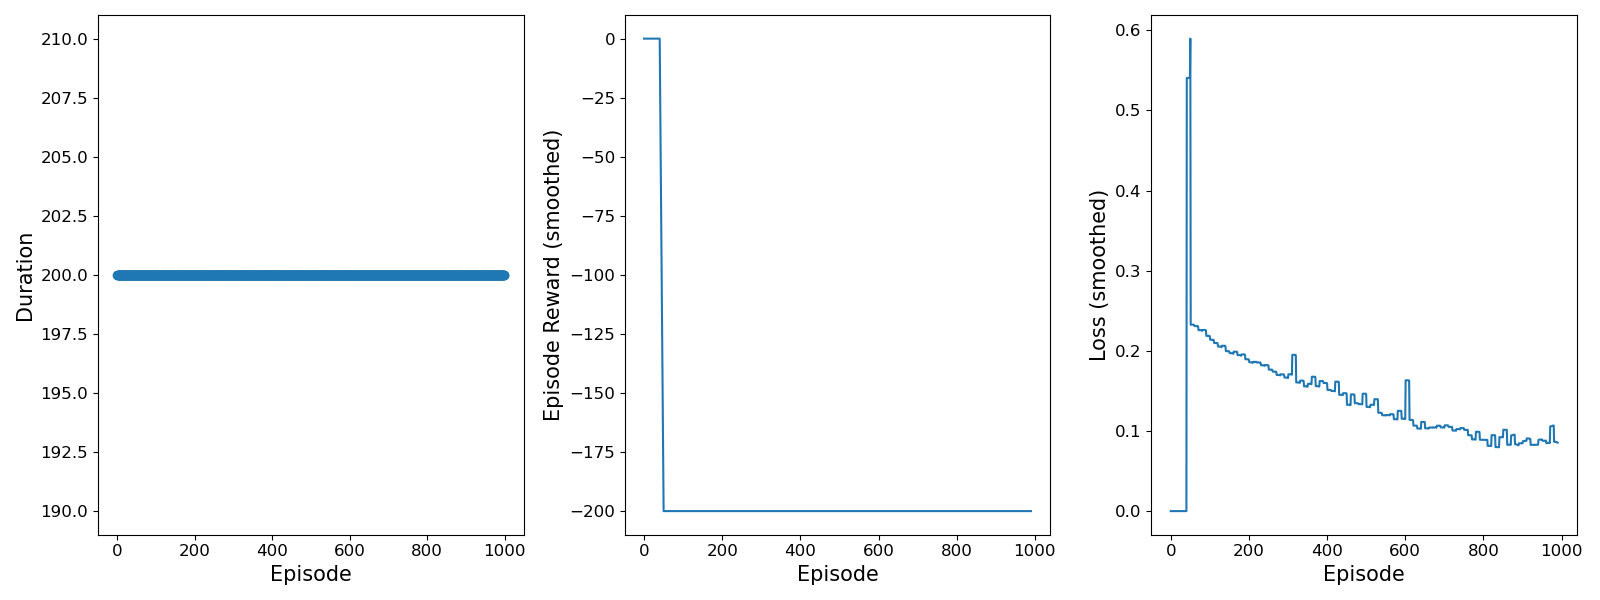
\includegraphics[width=.9\textwidth]{../runs/dqn_vanilla/up-tau=1/figs/full_results}
            \caption{Results associated to the training of a vanilla DQN agent.}
            \label{fig:dqn-vanilla-neps=1000}
        \end{figure}
        This is due again to the sparsity of the reward. 
        \subsection{Training metrics}
        To analyse further the training behaviour of our agents we can look at the loss and reward per episode. We can moreover look at the cumulative (cumulated) reward and cumulative successes over the episodes. 
        \subsection{Heuristic reward}
        \subsubsection{Heuristic reward function}
        \begin{wrapfigure}{r}{0.6\textwidth}
            \centering
            \vspace{-1em}
            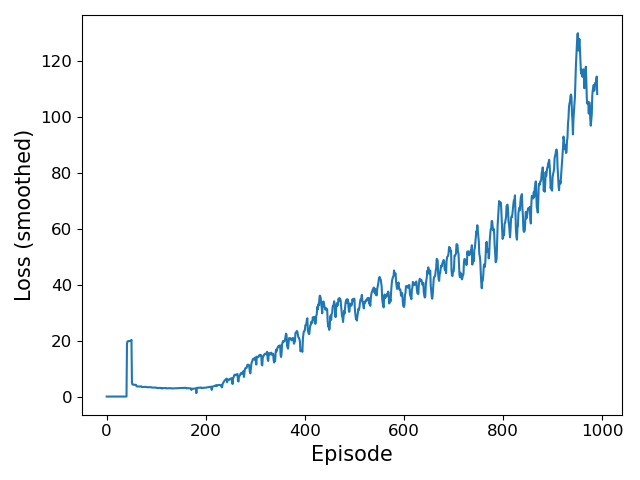
\includegraphics[width=0.6\textwidth]{../runs/dqn_heuristic/up-tau=3_d=2_frac=3.5/figs/loss}
            \caption{Evolution of cumulative training loss as a function of the episode for a heuristic reward agent. The reward factor is set to 3.5 and the loss is smoothed with a window of width 10.}
            \label{fig:dqn-heuristic-frac=3.5-loss}
        \end{wrapfigure}
        To alleviate the sparsity of the reward, we introduce a heuristic reward function which can be used as auxiliary reward for the DQN agent. Intuitively, we want this function to make the agent learn it should reach the top of the hill, which is placed on the right of the environnement. We therefore decide to take a heuristic function that assigns a reward if the agent is on the right of its (average) starting point. To make sure the agent tries and reach higher and higher on the hill, we decide to make this function be a growing one with the position. A simple and versatile proposal is to take 
        $$
        f(x) = A\mathbb I[x>\bar x\_0](x-\langle{x_0}\rangle)^n
        $$
        for $A>0$ some constant and a given $n\in\mathbb N^\star$. In practice we most often take $n=3$ and $A=0.1$. To make extra sure that for all values of the scale factor $A$, the agent does not get tempted to stay and collect the heuristic reward, we decide to offset the function by its maximal value (i.e. $A$). This way, the heuristic reward is always negative, and the agent is encouraged to reach the top of the hill.
        \begin{figure}[h!]
            \centering
            \vspace{0em}
            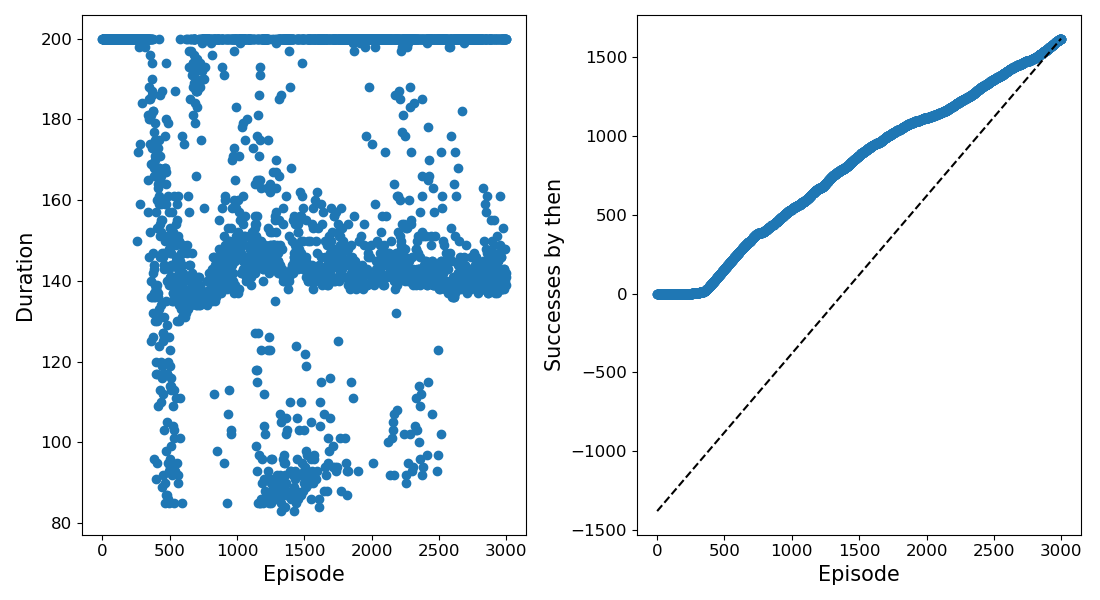
\includegraphics[width=.75\textwidth]{../runs/dqn_heuristic/up-tau=3_d=2_frac=3.5/figs/duration}
            \caption{Evolution of episode duration and cumulative number of successes as a function of the episode for a heuristic reward agent. The reward factor is set to 3.5.}
            \label{fig:dqn-heuristic-frac=3.5-duration}
        \end{figure}
        \begin{figure}[h!]
            \centering
            \vspace{0em}
            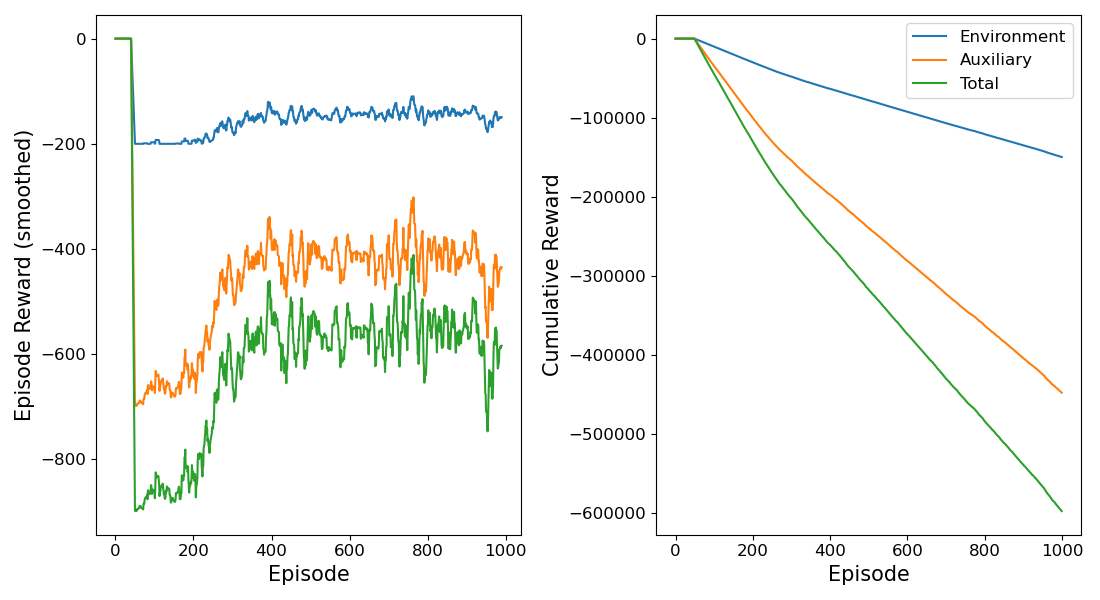
\includegraphics[width=.75\textwidth]{../runs/dqn_heuristic/up-tau=3_d=2_frac=3.5/figs/reward}
            \caption{Evolution of cumulative reward and cumulated cumulative reward (over the different episodes) as a function of the episode for a heuristic reward agent. The reward factor is set to 3.5 and the loss is smoothed with a window of width 10.}
            \label{fig:dqn-heuristic-frac=3.5-reward}
        \end{figure}
        \subsubsection{Auxiliary reward scaling}
        For the auxiliary reward to be useful, it should intuitively not be too small. Otherwise the situation would be almost the same as when no auxiliary reward is granted. As for the upper bound, things are more subtle. If the auxiliary reward is too large, it will dominate the environment reward. For the specific choice of heuristic reward, this should not impact the learning of the task, as by itself it would already lead the agent to the reward. However, it if one choses the reward unwisely, we can imagine that the agent could learn to stay on the right of the environment to collect reward rather than finishing the episode
        \begin{figure}[h!]
            \centering
            \vspace{0em}
            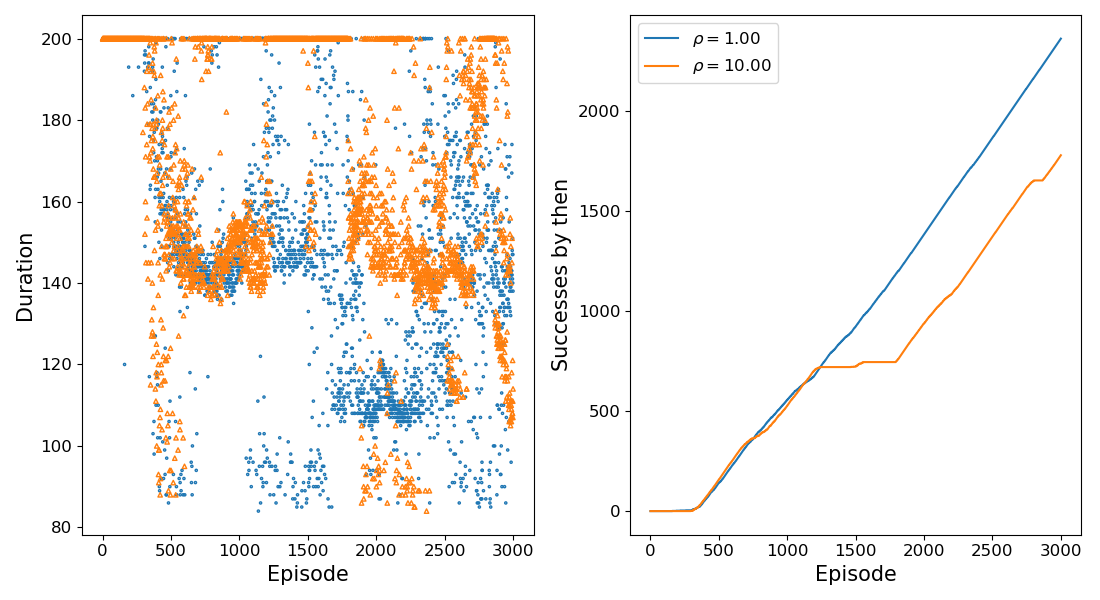
\includegraphics[width=.75\textwidth]{../runs/dqn_heuristic/comparison}
            \caption{Gamma GLM fit of the yearly maxima. Extreme events that occurred between 2013 and 2023 are also included.}
            \label{fig:dqn-heuristic-comparison}
        \end{figure}
        This intuition is confirmed by the results reported in fig ... . 
            %* test the higher reward with low degree func ? 
            %* be on the lookout for instabilities 
        \subsection{Two types of solutions ?}
        From the plot of the episode durations, we can see that the agent seems to have two distinct behaviours. Indeed, we can see that the density of points is larger for $90<d<120$ and $150<d<180$ than in between of these ranges. Investigating this more closely (inspecting the trajectories associated to these performances), one can trace this difference back to the initial condition. 
        
        If we start on the right of the minimum, we are able to reach the goal fast by only 2 large swings : the first to the left and the second to the right. If we start on the left of the minimum, the solution takes longer. Indeed, we need to go right, then left, then right again. This is due to the fact that the car has to gain enough speed to reach the top of the hill.
        Notice that the distinction between these two solutions is not that sharp. This is due to the fact that the initial condition is uniform over $[-0.6,-0.4]$, and so the agent sometimes starts close to the minimum, and therefore is not exactly in any of the two cases. 
        %Indeed, one could think that the optimal strategy would be to go right->left->right with as large swings as possible. However, doing so results in an unnecessary large (and time-consuming) left swing, since as seen in the first solution the first (non large) swing is sufficient to obtained the necessary speed. The 
        \section{RND reward}
            \subsection{Normalisation} 
            As recommended by the hint, we standardise the input and output of the RND network. The input standardisation is done since we want to output to vary as a function of how different the observed state is compared to the previously visited ones. Indeed, subtracting the typical state (i.e. the mean one) provides a good idea of how different the new input state is. The normalising by the typical distance from the mean state (i.e. the standard deviation) is done to make sure the input is of order 1, which is a good practice for neural networks to avoid instabilities.
            
            The standardisation of the output is instead done to make sure that we can control the characteristics of the RND reward attributed to the states. Indeed, by subtracting the mean we make sure that typical states are penalised  while new ones are rewarded (so we promote exploration); while normalisation make it possible to tweak the the order of magnitude of the reward (as normalised variables are of order 1). The clamping is done to avoid problems with the non-linearity of the neural network. 
            %    * but then why not the in Q net ? can't scale the environment to gain stability ?
            \subsection{Reward-factor scale}
            Mostly the same argument applies as for the heuristic reward. This time however, if the factor is taken too large, we expect the agent to prefer exploring instead of ending the episode by reaching the top of the hill. Indeed, when the agent will have reached the top of the hill a few times, the states that will have allowed it to do so will have a low RND reward. This is because the RND network will have seen them many times, and so the prediction error will be low.
            * right size ?
            * crude scale : over an episode the rewards should be comparable ?? 
            * handling gradients 
            * they are set to zero after each update
            * we use target network to only include part of the loss in the differenciation 
          * dataloaders are usually used for training (to shuffle data and create batches)
            * can't add samples to it, and should not re-define it from scratch 
              * we just keep a list instead, sampling with random indices 
          * we only start training once the replay buffer is full 
          * implementation of target net was done with help of chat gpt (command to import the weights from another net)
        \subsection{Comparison to heuristic reward}
        * difference in behaviour : we oscillate between the two possible solutions. This can be explained by the fact that the RND reward penalises the agent for repeating moves, and therefore leads the agent to switch its method more. 
    
        \section{Dyna}
        The Dyna algorithm relies on the discretization of the phase space (space of positions and velocities).
        The main parameter that will be varied in this section is this section is the size factor $\alpha$. We take as a reference of the step sizes the vector suggested in the project description ($\Delta x_0, \Delta v_0$) = (0.025, 0.005). We then test discretizations of the form ($\Delta x, \Delta v$) = $\alpha$ ($\Delta x_0, \Delta v_0$) 
        for different values of $\alpha$. Another parameter is the number $k$ of (state,action) pairs randomly sampled among all the visited state-action pairs. We fix it to $k=3$ and we will provide a note about it at the end of this section. 

        \subsection{Dyna manages to solve the task for some values of $\alpha$ !}
        When considering the original discrtization ($\alpha=1$), we observe that the task is solved, in the sense that successes (defined by episodes where the target is reached before 200 steps) are observed. 
        As in the previous sections, we plot the duration of each episode during the training, as well as the number of success with respect to the number of episodes. 
        In Figure ???, we show the result for $\alpha=1.5$ considered as a value allowing a good training (better than $\alpha=1$). We also plot results for values $\alpha=0.55$ and $\alpha=4.5$. 
        
        \begin{figure}[h]
            \centering
            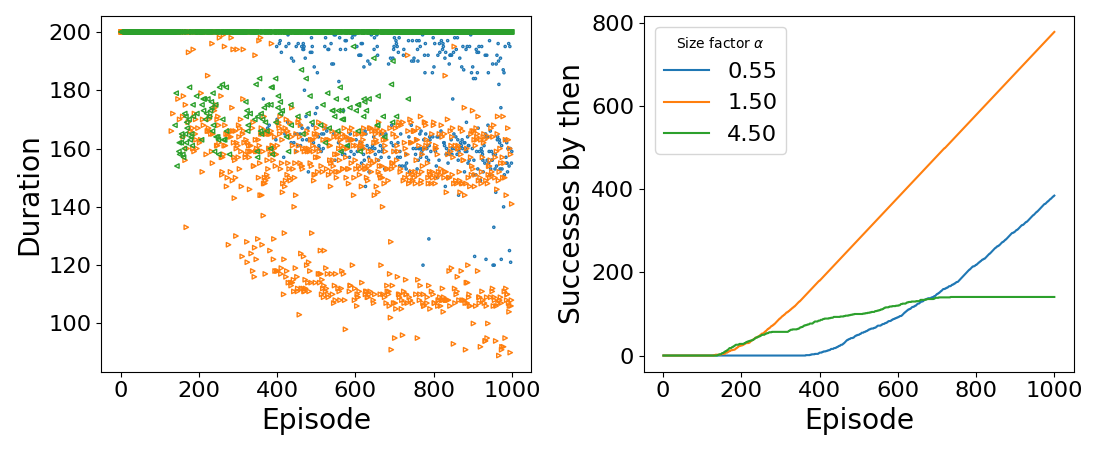
\includegraphics[width=0.9\textwidth]{../runs/dyna/dyna_comparison.png}
            \caption{}
        \end{figure}
        
        Value $\alpha=1.5$ shows a good performance as first successes are observed before 200 epsiodes. Then the line of success wrt to the number of epsiodes becomes, for higher number of episodes, a line of slope 1. Interestingly, for that discretuzation size, a pattern (that will be discussed later) appears. For a lower value $\alpha=0.55$ (fine grained discretization), performance is affected in the following way: the first successes are observed only after around 350 epsiodes, and the curve becomes a line of slope lower than 1 (meaning that even after a high number of iterations, some episodes are failures). 
        Value $\alpha=4.5$ also shows a low perfomance as the number of successes starts stagnating (less than 150 successes are observed after 1000 episodes). 
        For even too high values like $\alpha=8$, no success is observed in the window of the 1000 first episodes. This is due to the fact that ???.
        In the same way, for too low values like $\alpha=0.3$ no success is observed within the 1000 first episodes. Explanation ???. 
        % put the matrix of counts ? saying that it didnt explore much of the space ? 

       
        \begin{wrapfigure}{r}{0.6\textwidth}
            \centering
            \vspace{-1em}
            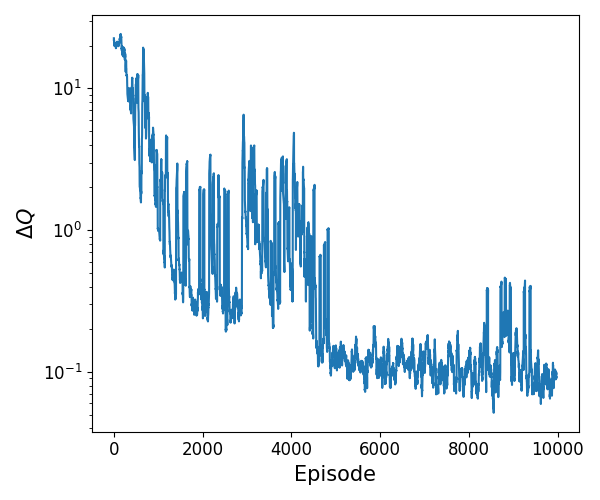
\includegraphics[width=0.6\textwidth]{../runs/dyna/dyna-k=3-ss_coef=1.5_eps=10000/figs/log_Q_value_changes.png}
            \caption{}
        \end{wrapfigure}

        At each episode one can compute the euclidean distance between the matrices $Q$ before and after the episode. This will provide a measure of the Q-value update. Figure ??? shows the evolution of that the Q-value update step for a simulation with 10000 episodes, using the most suitable value $\alpha=1.5$ among the ones that we have tested. As before, we consider $k=3$. Notice that the $y$-axis is in log-scale
        As expected, one can see that the Q-value update step overall decreases with the increase of the number of episodes. This indicates that the update equation: $Q(s,a) \leftarrow \hat{R}(s,a) + \gamma \sum_{s'} \hat{P}_{s,a}(s') \max_{a'}Q(s',a')$ is converging towards a fixed point. The decreasing is however not monotonic. Peaks are observed and correspond to moments at which the estimation of the $Q$ values undergoes a big change, corresponding to the agent learning new strategies (or perfecting). Notice that the decrease of $\Delta Q$ does not plateau at the last episodes (setting the $x$-axis to a log scale allows to see that the decrease continues).
        

        

        \subsection{Intuitive explanation on why it works}
        Having discretized the space, we dictate to the agent which action to take based on its projection on the grid of states. 
        The main advantage that this allows lies in the fact that 




        \subsection{$Q$ values table and characteristic trajectories}
        In the following, we show the estimation of the $Q$ values after the learning. In Figure \ref{Qmatrixcounts}, we represent for each state $s$ (located by a position and a velocity) the value $\max_a Q(s,a)$. On top, we represent three trajectories each corresponding to one the groups of episodes described above. 
        The second subplot indicated the set of states that have been visited (1 if visited and 0 if not). Last part of the figure shows the the number of times each of the states has been visited. Simulation done for 3000 episodes, $k=3$ and $\alpha=1.5$.
        We choose to represent the three trajectories in the same plot in order to save space in the report.

        \begin{figure}[h]
            \centering
            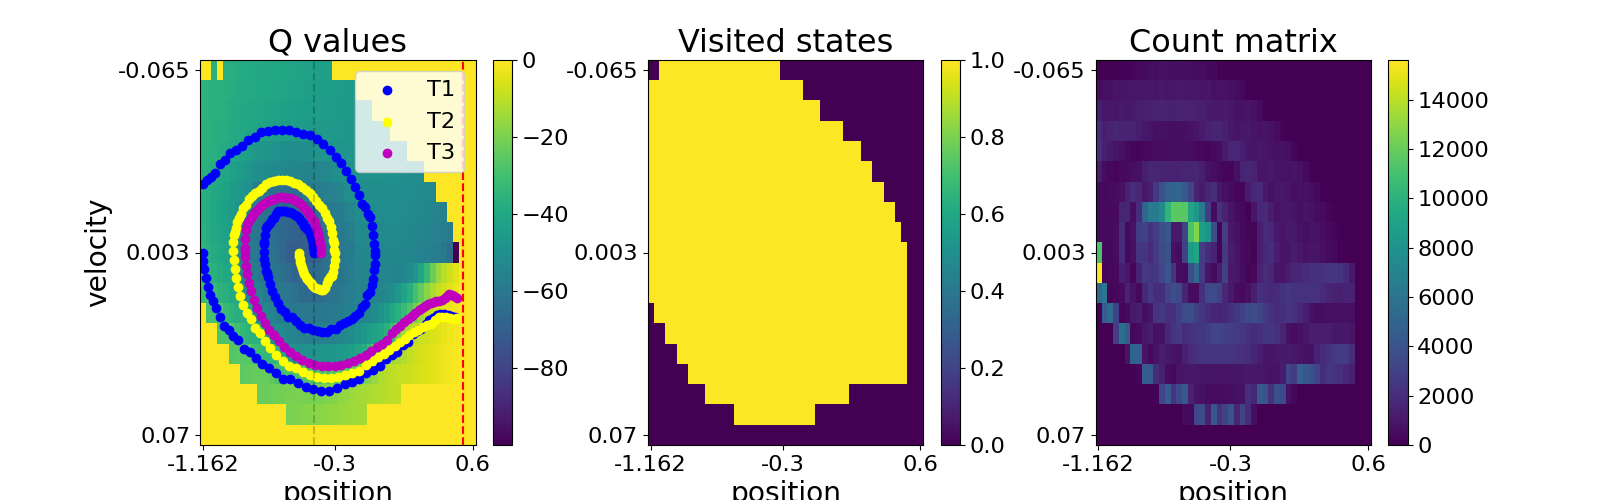
\includegraphics[width=1\textwidth]{../runs/dyna/dyna-k=3-ss_coef=1.5_eps=3000/figs/Q_final_matrix.png}
            \caption{Qmatrixcounts}
        \end{figure}

        Interestingly, the plot of $Q$-values shows a spiral starting at the bottom of the mountain and velocity 0. The spiraling behavior is followed by the trajectories represented. One can notice that in the lower part (positive velocities), when approaching to goal position, the $\max_a Q(s,a)$ values start approchaing zero values. This means that being present in those states, one would not expect to recieve a lot of negative reward before the end of the episode, in other words, the state easily leads to the goal.  
        % On the extreme left (and negative velocities), quantity $\max_a Q(s,a)$ has the same value, and this is due to the fact that all those states are "immediate predecessors" of the state on the extreme left position and velocity 0. This is because when the car hits the wall, its velocity immediately drops to zero. 
        Matrix of counts illustrates the fact that after 3000 epsiodes, most occupied states are disposed in spirals. Interestingly, a peak of count can be seen at the extreme left position and zero velocity, corresponding to cases where the car hits the wall. 

        

        \subsection{Bonus}
        \subsection{Note on varying $k$}

        \section{Conclusion}

        \section{Appendix}
\end{document}